
  
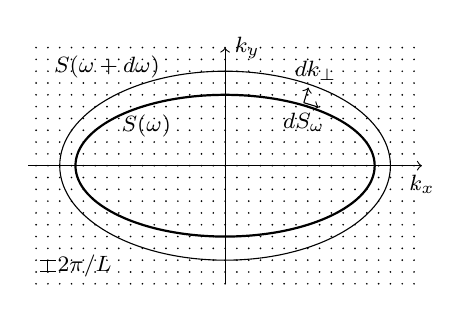
\begin{tikzpicture}[font=\footnotesize]

%\useasboundingbox (-1.3,-1.2) rectangle (11.2,4.7);
%	\draw (0,0) rectangle (5,4);

  
%\clip (-26mm,-16mm) rectangle  (26mm, 16mm);  
   
 \foreach \u in {-16,-15,...,16}{%  
     \foreach \v in {-10,-9,...,10}{%  
          \draw[fill=gray]  (\u * 1.5mm,\v * 1.5mm)  circle (0.02mm) ;  
     }
  }
  
   \draw [ |-| ] ( -15 * 1.5mm, -9 * 1.5mm) -- node[right] { $2 \pi / L$} ++ (0, 1.5mm);
  
  
\draw[->] (-2.5,0) -- (2.5,0) node [below] {$k_x$};  
  \draw[->] (0,-1.5) -- (0,1.5) node [right] {$k_y$};  

\draw[thick] (0,0) ellipse (1.9cm and 0.9cm);
\draw[] (0,0) ellipse (2.1cm and 1.2cm);

\node at (-10mm, 5mm) {$S(\omega)$};
\node at (-15mm, 12.5mm) {$S(\omega + d\omega)$};


\draw[->] (10mm,8mm) -- node (a) {} ++ (73:2mm);
\draw[->] (10mm,8mm) -- ++ (-17:2mm);

\node at (11.5mm, 12mm) {$dk_\perp$};
\node at (10mm, 5.5mm) {$dS_\omega$};



  
  \end{tikzpicture}



